\documentclass[1p]{elsarticle_modified}
%\bibliographystyle{elsarticle-num}

%\usepackage[colorlinks]{hyperref}
%\usepackage{abbrmath_seonhwa} %\Abb, \Ascr, \Acal ,\Abf, \Afrak
\usepackage{amsfonts}
\usepackage{amssymb}
\usepackage{amsmath}
\usepackage{amsthm}
\usepackage{scalefnt}
\usepackage{amsbsy}
\usepackage{kotex}
\usepackage{caption}
\usepackage{subfig}
\usepackage{color}
\usepackage{graphicx}
\usepackage{xcolor} %% white, black, red, green, blue, cyan, magenta, yellow
\usepackage{float}
\usepackage{setspace}
\usepackage{hyperref}

\usepackage{tikz}
\usetikzlibrary{arrows}

\usepackage{multirow}
\usepackage{array} % fixed length table
\usepackage{hhline}

%%%%%%%%%%%%%%%%%%%%%
\makeatletter
\renewcommand*\env@matrix[1][\arraystretch]{%
	\edef\arraystretch{#1}%
	\hskip -\arraycolsep
	\let\@ifnextchar\new@ifnextchar
	\array{*\c@MaxMatrixCols c}}
\makeatother %https://tex.stackexchange.com/questions/14071/how-can-i-increase-the-line-spacing-in-a-matrix
%%%%%%%%%%%%%%%

\usepackage[normalem]{ulem}

\newcommand{\msout}[1]{\ifmmode\text{\sout{\ensuremath{#1}}}\else\sout{#1}\fi}
%SOURCE: \msout is \stkout macro in https://tex.stackexchange.com/questions/20609/strikeout-in-math-mode

\newcommand{\cancel}[1]{
	\ifmmode
	{\color{red}\msout{#1}}
	\else
	{\color{red}\sout{#1}}
	\fi
}

\newcommand{\add}[1]{
	{\color{blue}\uwave{#1}}
}

\newcommand{\replace}[2]{
	\ifmmode
	{\color{red}\msout{#1}}{\color{blue}\uwave{#2}}
	\else
	{\color{red}\sout{#1}}{\color{blue}\uwave{#2}}
	\fi
}

\newcommand{\Sol}{\mathcal{S}} %segment
\newcommand{\D}{D} %diagram
\newcommand{\A}{\mathcal{A}} %arc


%%%%%%%%%%%%%%%%%%%%%%%%%%%%%5 test

\def\sl{\operatorname{\textup{SL}}(2,\Cbb)}
\def\psl{\operatorname{\textup{PSL}}(2,\Cbb)}
\def\quan{\mkern 1mu \triangleright \mkern 1mu}

\theoremstyle{definition}
\newtheorem{thm}{Theorem}[section]
\newtheorem{prop}[thm]{Proposition}
\newtheorem{lem}[thm]{Lemma}
\newtheorem{ques}[thm]{Question}
\newtheorem{cor}[thm]{Corollary}
\newtheorem{defn}[thm]{Definition}
\newtheorem{exam}[thm]{Example}
\newtheorem{rmk}[thm]{Remark}
\newtheorem{alg}[thm]{Algorithm}

\newcommand{\I}{\sqrt{-1}}
\begin{document}

%\begin{frontmatter}
%
%\title{Boundary parabolic representations of knots up to 8 crossings}
%
%%% Group authors per affiliation:
%\author{Yunhi Cho} 
%\address{Department of Mathematics, University of Seoul, Seoul, Korea}
%\ead{yhcho@uos.ac.kr}
%
%
%\author{Seonhwa Kim} %\fnref{s_kim}}
%\address{Center for Geometry and Physics, Institute for Basic Science, Pohang, 37673, Korea}
%\ead{ryeona17@ibs.re.kr}
%
%\author{Hyuk Kim}
%\address{Department of Mathematical Sciences, Seoul National University, Seoul 08826, Korea}
%\ead{hyukkim@snu.ac.kr}
%
%\author{Seokbeom Yoon}
%\address{Department of Mathematical Sciences, Seoul National University, Seoul, 08826,  Korea}
%\ead{sbyoon15@snu.ac.kr}
%
%\begin{abstract}
%We find all boundary parabolic representation of knots up to 8 crossings.
%
%\end{abstract}
%\begin{keyword}
%    \MSC[2010] 57M25 
%\end{keyword}
%
%\end{frontmatter}

%\linenumbers
%\tableofcontents
%
\newcommand\colored[1]{\textcolor{white}{\rule[-0.35ex]{0.8em}{1.4ex}}\kern-0.8em\color{red} #1}%
%\newcommand\colored[1]{\textcolor{white}{ #1}\kern-2.17ex	\textcolor{white}{ #1}\kern-1.81ex	\textcolor{white}{ #1}\kern-2.15ex\color{red}#1	}

{\Large $\underline{12a_{0086}~(K12a_{0086})}$}

\setlength{\tabcolsep}{10pt}
\renewcommand{\arraystretch}{1.6}
\vspace{1cm}\begin{tabular}{m{100pt}>{\centering\arraybackslash}m{274pt}}
\multirow{5}{120pt}{
	\centering
	\includegraphics[width=112pt]{../../../GIT/diagram.site/Diagrams/png/887_12a_0086.png}\\
\ \ \ A knot diagram\footnotemark}&
\allowdisplaybreaks
\textbf{Linearized knot diagam} \\
\cline{2-2}
 &
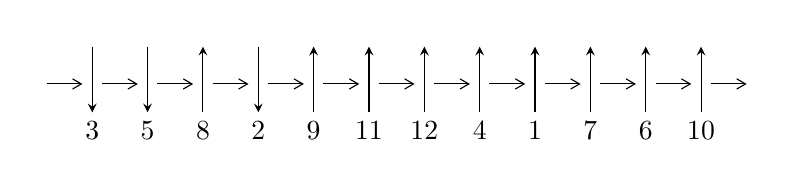
\begin{tikzpicture}[x=20pt, y=17pt]
	% nodes
	\node (C0) at (0, 0) {};
	\node (C1) at (1, 0) {};
	\node (C1U) at (1, +1) {};
	\node (C1D) at (1, -1) {3};

	\node (C2) at (2, 0) {};
	\node (C2U) at (2, +1) {};
	\node (C2D) at (2, -1) {5};

	\node (C3) at (3, 0) {};
	\node (C3U) at (3, +1) {};
	\node (C3D) at (3, -1) {8};

	\node (C4) at (4, 0) {};
	\node (C4U) at (4, +1) {};
	\node (C4D) at (4, -1) {2};

	\node (C5) at (5, 0) {};
	\node (C5U) at (5, +1) {};
	\node (C5D) at (5, -1) {9};

	\node (C6) at (6, 0) {};
	\node (C6U) at (6, +1) {};
	\node (C6D) at (6, -1) {11};

	\node (C7) at (7, 0) {};
	\node (C7U) at (7, +1) {};
	\node (C7D) at (7, -1) {12};

	\node (C8) at (8, 0) {};
	\node (C8U) at (8, +1) {};
	\node (C8D) at (8, -1) {4};

	\node (C9) at (9, 0) {};
	\node (C9U) at (9, +1) {};
	\node (C9D) at (9, -1) {1};

	\node (C10) at (10, 0) {};
	\node (C10U) at (10, +1) {};
	\node (C10D) at (10, -1) {7};

	\node (C11) at (11, 0) {};
	\node (C11U) at (11, +1) {};
	\node (C11D) at (11, -1) {6};

	\node (C12) at (12, 0) {};
	\node (C12U) at (12, +1) {};
	\node (C12D) at (12, -1) {10};
	\node (C13) at (13, 0) {};

	% arrows
	\draw[->,>={angle 60}]
	(C0) edge (C1) (C1) edge (C2) (C2) edge (C3) (C3) edge (C4) (C4) edge (C5) (C5) edge (C6) (C6) edge (C7) (C7) edge (C8) (C8) edge (C9) (C9) edge (C10) (C10) edge (C11) (C11) edge (C12) (C12) edge (C13) ;	\draw[->,>=stealth]
	(C1U) edge (C1D) (C2U) edge (C2D) (C3D) edge (C3U) (C4U) edge (C4D) (C5D) edge (C5U) (C6D) edge (C6U) (C7D) edge (C7U) (C8D) edge (C8U) (C9D) edge (C9U) (C10D) edge (C10U) (C11D) edge (C11U) (C12D) edge (C12U) ;
	\end{tikzpicture} \\
\hhline{~~} \\& 
\textbf{Solving Sequence} \\ \cline{2-2} 
 &
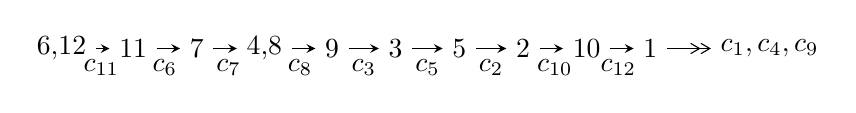
\begin{tikzpicture}[x=23pt, y=7pt]
	% node
	\node (A0) at (-1/8, 0) {6,12};
	\node (A1) at (1, 0) {11};
	\node (A2) at (2, 0) {7};
	\node (A3) at (49/16, 0) {4,8};
	\node (A4) at (33/8, 0) {9};
	\node (A5) at (41/8, 0) {3};
	\node (A6) at (49/8, 0) {5};
	\node (A7) at (57/8, 0) {2};
	\node (A8) at (65/8, 0) {10};
	\node (A9) at (73/8, 0) {1};
	\node (C1) at (1/2, -1) {$c_{11}$};
	\node (C2) at (3/2, -1) {$c_{6}$};
	\node (C3) at (5/2, -1) {$c_{7}$};
	\node (C4) at (29/8, -1) {$c_{8}$};
	\node (C5) at (37/8, -1) {$c_{3}$};
	\node (C6) at (45/8, -1) {$c_{5}$};
	\node (C7) at (53/8, -1) {$c_{2}$};
	\node (C8) at (61/8, -1) {$c_{10}$};
	\node (C9) at (69/8, -1) {$c_{12}$};
	\node (A10) at (11, 0) {$c_{1},c_{4},c_{9}$};

	% edge
	\draw[->,>=stealth]	
	(A0) edge (A1) (A1) edge (A2) (A2) edge (A3) (A3) edge (A4) (A4) edge (A5) (A5) edge (A6) (A6) edge (A7) (A7) edge (A8) (A8) edge (A9) ;
	\draw[->>,>={angle 60}]	
	(A9) edge (A10);
\end{tikzpicture} \\ 

\end{tabular} \\

\footnotetext{
The image of knot diagram is generated by the software ``\textbf{Draw programme}" developed by Andrew Bartholomew(\url{http://www.layer8.co.uk/maths/draw/index.htm\#Running-draw}), where we modified some parts for our purpose(\url{https://github.com/CATsTAILs/LinksPainter}).
}\phantom \\ \newline 
\centering \textbf{Ideals for irreducible components\footnotemark of $X_{\text{par}}$} 
 
\begin{align*}
I^u_{1}&=\langle 
- u^{90}+u^{89}+\cdots+3 u^2+b,\;- u^{88}+u^{87}+\cdots+a-3 u,\;u^{92}-2 u^{91}+\cdots+3 u-1\rangle \\
I^u_{2}&=\langle 
- u^2+b-1,\;- u^2+a-2,\;u^3+2 u-1\rangle \\
I^u_{3}&=\langle 
u^3+u^2+b+u+1,\;u^3+u^2+a+2 u+2,\;u^4+u^3+2 u^2+2 u+1\rangle \\
\\
\end{align*}
\raggedright * 3 irreducible components of $\dim_{\mathbb{C}}=0$, with total 99 representations.\\
\footnotetext{All coefficients of polynomials are rational numbers. But the coefficients are sometimes approximated in decimal forms when there is not enough margin.}
\newpage
\renewcommand{\arraystretch}{1}
\centering \section*{I. $I^u_{1}= \langle - u^{90}+u^{89}+\cdots+3 u^2+b,\;- u^{88}+u^{87}+\cdots+a-3 u,\;u^{92}-2 u^{91}+\cdots+3 u-1 \rangle$}
\flushleft \textbf{(i) Arc colorings}\\
\begin{tabular}{m{7pt} m{180pt} m{7pt} m{180pt} }
\flushright $a_{6}=$&$\begin{pmatrix}0\\u\end{pmatrix}$ \\
\flushright $a_{12}=$&$\begin{pmatrix}1\\0\end{pmatrix}$ \\
\flushright $a_{11}=$&$\begin{pmatrix}1\\u^2\end{pmatrix}$ \\
\flushright $a_{7}=$&$\begin{pmatrix}u\\u^3+u\end{pmatrix}$ \\
\flushright $a_{4}=$&$\begin{pmatrix}u^{88}- u^{87}+\cdots-6 u^2+3 u\\u^{90}- u^{89}+\cdots+6 u^3-3 u^2\end{pmatrix}$ \\
\flushright $a_{8}=$&$\begin{pmatrix}u^3+2 u\\u^3+u\end{pmatrix}$ \\
\flushright $a_{9}=$&$\begin{pmatrix}u^{10}+5 u^8+8 u^6+3 u^4- u^2+1\\u^{12}+6 u^{10}+12 u^8+8 u^6+u^4+2 u^2\end{pmatrix}$ \\
\flushright $a_{3}=$&$\begin{pmatrix}2 u^{88}- u^{87}+\cdots+4 u-1\\u^{89}+u^{88}+\cdots-2 u^2- u\end{pmatrix}$ \\
\flushright $a_{5}=$&$\begin{pmatrix}- u^{21}-10 u^{19}+\cdots+2 u^3- u\\- u^{23}-11 u^{21}+\cdots-2 u^3+u\end{pmatrix}$ \\
\flushright $a_{2}=$&$\begin{pmatrix}u^{88}- u^{87}+\cdots-6 u^2+3 u\\u^{88}- u^{87}+\cdots+5 u^3-3 u^2\end{pmatrix}$ \\
\flushright $a_{10}=$&$\begin{pmatrix}u^2+1\\u^4+2 u^2\end{pmatrix}$ \\
\flushright $a_{1}=$&$\begin{pmatrix}- u^6-3 u^4-2 u^2+1\\- u^8-4 u^6-4 u^4\end{pmatrix}$\\&\end{tabular}
\flushleft \textbf{(ii) Obstruction class $= -1$}\\~\\
\flushleft \textbf{(iii) Cusp Shapes $= 4 u^{91}-8 u^{90}+\cdots-5 u+15$}\\~\\
\newpage\renewcommand{\arraystretch}{1}
\flushleft \textbf{(iv) u-Polynomials at the component}\newline \\
\begin{tabular}{m{50pt}|m{274pt}}
Crossings & \hspace{64pt}u-Polynomials at each crossing \\
\hline $$\begin{aligned}c_{1}\end{aligned}$$&$\begin{aligned}
&u^{92}+44 u^{91}+\cdots+78 u+1
\end{aligned}$\\
\hline $$\begin{aligned}c_{2},c_{4}\end{aligned}$$&$\begin{aligned}
&u^{92}-8 u^{91}+\cdots+14 u-1
\end{aligned}$\\
\hline $$\begin{aligned}c_{3},c_{8}\end{aligned}$$&$\begin{aligned}
&u^{92}+u^{91}+\cdots+192 u+128
\end{aligned}$\\
\hline $$\begin{aligned}c_{5}\end{aligned}$$&$\begin{aligned}
&u^{92}-2 u^{91}+\cdots+13397 u-11981
\end{aligned}$\\
\hline $$\begin{aligned}c_{6},c_{10},c_{11}\end{aligned}$$&$\begin{aligned}
&u^{92}-2 u^{91}+\cdots+3 u-1
\end{aligned}$\\
\hline $$\begin{aligned}c_{7}\end{aligned}$$&$\begin{aligned}
&u^{92}+2 u^{91}+\cdots+19896 u-4360
\end{aligned}$\\
\hline $$\begin{aligned}c_{9},c_{12}\end{aligned}$$&$\begin{aligned}
&u^{92}+14 u^{91}+\cdots+3115 u+131
\end{aligned}$\\
\hline
\end{tabular}\\~\\
\newpage\renewcommand{\arraystretch}{1}
\flushleft \textbf{(v) Riley Polynomials at the component}\newline \\
\begin{tabular}{m{50pt}|m{274pt}}
Crossings & \hspace{64pt}Riley Polynomials at each crossing \\
\hline $$\begin{aligned}c_{1}\end{aligned}$$&$\begin{aligned}
&y^{92}+16 y^{91}+\cdots-5674 y+1
\end{aligned}$\\
\hline $$\begin{aligned}c_{2},c_{4}\end{aligned}$$&$\begin{aligned}
&y^{92}-44 y^{91}+\cdots-78 y+1
\end{aligned}$\\
\hline $$\begin{aligned}c_{3},c_{8}\end{aligned}$$&$\begin{aligned}
&y^{92}-45 y^{91}+\cdots-438272 y+16384
\end{aligned}$\\
\hline $$\begin{aligned}c_{5}\end{aligned}$$&$\begin{aligned}
&y^{92}-10 y^{91}+\cdots+378763105 y+143544361
\end{aligned}$\\
\hline $$\begin{aligned}c_{6},c_{10},c_{11}\end{aligned}$$&$\begin{aligned}
&y^{92}+86 y^{91}+\cdots+y+1
\end{aligned}$\\
\hline $$\begin{aligned}c_{7}\end{aligned}$$&$\begin{aligned}
&y^{92}+30 y^{91}+\cdots+525356144 y+19009600
\end{aligned}$\\
\hline $$\begin{aligned}c_{9},c_{12}\end{aligned}$$&$\begin{aligned}
&y^{92}+74 y^{91}+\cdots+260373 y+17161
\end{aligned}$\\
\hline
\end{tabular}\\~\\
\newpage\flushleft \textbf{(vi) Complex Volumes and Cusp Shapes}
$$\begin{array}{c|c|c}  
\text{Solutions to }I^u_{1}& \I (\text{vol} + \sqrt{-1}CS) & \text{Cusp shape}\\
 \hline 
\begin{aligned}
u &= -0.153909 + 1.134970 I \\
a &= \phantom{-}0.417347 + 1.214000 I \\
b &= \phantom{-}1.49588 - 1.44581 I\end{aligned}
 & \phantom{-}1.12873 + 4.25478 I & \phantom{-0.000000 } 0 \\ \hline\begin{aligned}
u &= -0.153909 - 1.134970 I \\
a &= \phantom{-}0.417347 - 1.214000 I \\
b &= \phantom{-}1.49588 + 1.44581 I\end{aligned}
 & \phantom{-}1.12873 - 4.25478 I & \phantom{-0.000000 } 0 \\ \hline\begin{aligned}
u &= -0.178162 + 1.177710 I \\
a &= -0.495039 - 1.310920 I \\
b &= -1.68518 + 1.60196 I\end{aligned}
 & \phantom{-}2.58467 - 1.25382 I & \phantom{-0.000000 } 0 \\ \hline\begin{aligned}
u &= -0.178162 - 1.177710 I \\
a &= -0.495039 + 1.310920 I \\
b &= -1.68518 - 1.60196 I\end{aligned}
 & \phantom{-}2.58467 + 1.25382 I & \phantom{-0.000000 } 0 \\ \hline\begin{aligned}
u &= \phantom{-}0.692151 + 0.390660 I \\
a &= -2.83083 + 0.45729 I \\
b &= -2.42917 + 0.16265 I\end{aligned}
 & -1.15801 + 12.77270 I & \phantom{-}5.19545 - 9.98793 I \\ \hline\begin{aligned}
u &= \phantom{-}0.692151 - 0.390660 I \\
a &= -2.83083 - 0.45729 I \\
b &= -2.42917 - 0.16265 I\end{aligned}
 & -1.15801 - 12.77270 I & \phantom{-}5.19545 + 9.98793 I \\ \hline\begin{aligned}
u &= -0.655533 + 0.444833 I \\
a &= -0.568758 + 0.309874 I \\
b &= -0.165875 + 0.683566 I\end{aligned}
 & -4.78712 - 0.77055 I & \phantom{-}4.27518 - 2.02219 I \\ \hline\begin{aligned}
u &= -0.655533 - 0.444833 I \\
a &= -0.568758 - 0.309874 I \\
b &= -0.165875 - 0.683566 I\end{aligned}
 & -4.78712 + 0.77055 I & \phantom{-}4.27518 + 2.02219 I \\ \hline\begin{aligned}
u &= -0.622505 + 0.481239 I \\
a &= \phantom{-}0.245787 - 0.637722 I \\
b &= -0.380467 - 0.619541 I\end{aligned}
 & -4.93263 - 3.45869 I & \phantom{-}3.45815 + 8.17533 I \\ \hline\begin{aligned}
u &= -0.622505 - 0.481239 I \\
a &= \phantom{-}0.245787 + 0.637722 I \\
b &= -0.380467 + 0.619541 I\end{aligned}
 & -4.93263 + 3.45869 I & \phantom{-}3.45815 - 8.17533 I\\
 \hline 
 \end{array}$$\newpage$$\begin{array}{c|c|c}  
\text{Solutions to }I^u_{1}& \I (\text{vol} + \sqrt{-1}CS) & \text{Cusp shape}\\
 \hline 
\begin{aligned}
u &= \phantom{-}0.681826 + 0.378269 I \\
a &= \phantom{-}2.73645 - 0.17651 I \\
b &= \phantom{-}2.29636 - 0.07821 I\end{aligned}
 & \phantom{-}1.22083 + 7.21067 I & \phantom{-}8.33989 - 6.35791 I \\ \hline\begin{aligned}
u &= \phantom{-}0.681826 - 0.378269 I \\
a &= \phantom{-}2.73645 + 0.17651 I \\
b &= \phantom{-}2.29636 + 0.07821 I\end{aligned}
 & \phantom{-}1.22083 - 7.21067 I & \phantom{-}8.33989 + 6.35791 I \\ \hline\begin{aligned}
u &= \phantom{-}0.555518 + 0.540981 I \\
a &= -1.11207 + 2.49940 I \\
b &= -0.953299 + 0.378073 I\end{aligned}
 & -1.75174 - 8.58830 I & \phantom{-}3.72994 + 4.13812 I \\ \hline\begin{aligned}
u &= \phantom{-}0.555518 - 0.540981 I \\
a &= -1.11207 - 2.49940 I \\
b &= -0.953299 - 0.378073 I\end{aligned}
 & -1.75174 + 8.58830 I & \phantom{-}3.72994 - 4.13812 I \\ \hline\begin{aligned}
u &= -0.666620 + 0.388015 I \\
a &= -0.958765 - 0.000505 I \\
b &= -0.754029 + 0.679010 I\end{aligned}
 & -3.47583 - 6.55474 I & \phantom{-}3.56008 + 7.35236 I \\ \hline\begin{aligned}
u &= -0.666620 - 0.388015 I \\
a &= -0.958765 + 0.000505 I \\
b &= -0.754029 - 0.679010 I\end{aligned}
 & -3.47583 + 6.55474 I & \phantom{-}3.56008 - 7.35236 I \\ \hline\begin{aligned}
u &= \phantom{-}0.145987 + 1.225320 I \\
a &= \phantom{-}0.007933 + 0.249436 I \\
b &= \phantom{-}0.748621 - 0.760668 I\end{aligned}
 & -2.36582 + 0.77393 I & \phantom{-0.000000 } 0 \\ \hline\begin{aligned}
u &= \phantom{-}0.145987 - 1.225320 I \\
a &= \phantom{-}0.007933 - 0.249436 I \\
b &= \phantom{-}0.748621 + 0.760668 I\end{aligned}
 & -2.36582 - 0.77393 I & \phantom{-0.000000 } 0 \\ \hline\begin{aligned}
u &= \phantom{-}0.651996 + 0.392636 I \\
a &= -3.32272 - 0.41767 I \\
b &= -2.40704 - 0.36202 I\end{aligned}
 & -4.32011 + 3.99543 I & \phantom{-}4.12422 - 6.59810 I \\ \hline\begin{aligned}
u &= \phantom{-}0.651996 - 0.392636 I \\
a &= -3.32272 + 0.41767 I \\
b &= -2.40704 + 0.36202 I\end{aligned}
 & -4.32011 - 3.99543 I & \phantom{-}4.12422 + 6.59810 I\\
 \hline 
 \end{array}$$\newpage$$\begin{array}{c|c|c}  
\text{Solutions to }I^u_{1}& \I (\text{vol} + \sqrt{-1}CS) & \text{Cusp shape}\\
 \hline 
\begin{aligned}
u &= \phantom{-}0.529646 + 0.527281 I \\
a &= \phantom{-}0.83363 - 2.44550 I \\
b &= \phantom{-}0.670451 - 0.398275 I\end{aligned}
 & \phantom{-}0.59744 - 3.14929 I & \phantom{-}6.80686 + 0.31636 I \\ \hline\begin{aligned}
u &= \phantom{-}0.529646 - 0.527281 I \\
a &= \phantom{-}0.83363 + 2.44550 I \\
b &= \phantom{-}0.670451 + 0.398275 I\end{aligned}
 & \phantom{-}0.59744 + 3.14929 I & \phantom{-}6.80686 - 0.31636 I \\ \hline\begin{aligned}
u &= -0.545896 + 0.498041 I \\
a &= -0.053053 - 0.997688 I \\
b &= -0.841966 - 0.459143 I\end{aligned}
 & -3.96124 + 2.53513 I & \phantom{-}1.92062 - 0.95185 I \\ \hline\begin{aligned}
u &= -0.545896 - 0.498041 I \\
a &= -0.053053 + 0.997688 I \\
b &= -0.841966 + 0.459143 I\end{aligned}
 & -3.96124 - 2.53513 I & \phantom{-}1.92062 + 0.95185 I \\ \hline\begin{aligned}
u &= -0.625833 + 0.381321 I \\
a &= \phantom{-}0.834785 + 0.303156 I \\
b &= \phantom{-}0.802569 - 0.344086 I\end{aligned}
 & -1.98725 - 2.24402 I & \phantom{-}5.47486 + 2.60472 I \\ \hline\begin{aligned}
u &= -0.625833 - 0.381321 I \\
a &= \phantom{-}0.834785 - 0.303156 I \\
b &= \phantom{-}0.802569 + 0.344086 I\end{aligned}
 & -1.98725 + 2.24402 I & \phantom{-}5.47486 - 2.60472 I \\ \hline\begin{aligned}
u &= \phantom{-}0.556284 + 0.474387 I \\
a &= -0.38833 + 3.14529 I \\
b &= -0.480167 + 1.085090 I\end{aligned}
 & -4.69977 - 0.02977 I & \phantom{-}2.52437 + 0.10755 I \\ \hline\begin{aligned}
u &= \phantom{-}0.556284 - 0.474387 I \\
a &= -0.38833 - 3.14529 I \\
b &= -0.480167 - 1.085090 I\end{aligned}
 & -4.69977 + 0.02977 I & \phantom{-}2.52437 - 0.10755 I \\ \hline\begin{aligned}
u &= -0.220636 + 1.250340 I \\
a &= -0.44070 - 1.47175 I \\
b &= -2.06377 + 1.59068 I\end{aligned}
 & \phantom{-}1.98043 - 5.03762 I & \phantom{-0.000000 } 0 \\ \hline\begin{aligned}
u &= -0.220636 - 1.250340 I \\
a &= -0.44070 + 1.47175 I \\
b &= -2.06377 - 1.59068 I\end{aligned}
 & \phantom{-}1.98043 + 5.03762 I & \phantom{-0.000000 } 0\\
 \hline 
 \end{array}$$\newpage$$\begin{array}{c|c|c}  
\text{Solutions to }I^u_{1}& \I (\text{vol} + \sqrt{-1}CS) & \text{Cusp shape}\\
 \hline 
\begin{aligned}
u &= -0.164083 + 1.261680 I \\
a &= \phantom{-}0.65175 + 1.65425 I \\
b &= \phantom{-}2.23983 - 2.06975 I\end{aligned}
 & -4.01978 - 2.64901 I & \phantom{-0.000000 } 0 \\ \hline\begin{aligned}
u &= -0.164083 - 1.261680 I \\
a &= \phantom{-}0.65175 - 1.65425 I \\
b &= \phantom{-}2.23983 + 2.06975 I\end{aligned}
 & -4.01978 + 2.64901 I & \phantom{-0.000000 } 0 \\ \hline\begin{aligned}
u &= \phantom{-}0.192419 + 1.262480 I \\
a &= \phantom{-}0.0551400 - 0.1149010 I \\
b &= -1.019200 + 0.512780 I\end{aligned}
 & -2.86556 + 4.87473 I & \phantom{-0.000000 } 0 \\ \hline\begin{aligned}
u &= \phantom{-}0.192419 - 1.262480 I \\
a &= \phantom{-}0.0551400 + 0.1149010 I \\
b &= -1.019200 - 0.512780 I\end{aligned}
 & -2.86556 - 4.87473 I & \phantom{-0.000000 } 0 \\ \hline\begin{aligned}
u &= \phantom{-}0.646126 + 0.313529 I \\
a &= \phantom{-}1.75378 + 0.37623 I \\
b &= \phantom{-}1.56532 - 0.11169 I\end{aligned}
 & \phantom{-}3.18820 + 3.73788 I & \phantom{-}10.37835 - 6.18860 I \\ \hline\begin{aligned}
u &= \phantom{-}0.646126 - 0.313529 I \\
a &= \phantom{-}1.75378 - 0.37623 I \\
b &= \phantom{-}1.56532 + 0.11169 I\end{aligned}
 & \phantom{-}3.18820 - 3.73788 I & \phantom{-}10.37835 + 6.18860 I \\ \hline\begin{aligned}
u &= -0.233887 + 1.270730 I \\
a &= \phantom{-}0.39170 + 1.45839 I \\
b &= \phantom{-}2.08527 - 1.50862 I\end{aligned}
 & \phantom{-}0.05201 - 10.63290 I & \phantom{-0.000000 } 0 \\ \hline\begin{aligned}
u &= -0.233887 - 1.270730 I \\
a &= \phantom{-}0.39170 - 1.45839 I \\
b &= \phantom{-}2.08527 + 1.50862 I\end{aligned}
 & \phantom{-}0.05201 + 10.63290 I & \phantom{-0.000000 } 0 \\ \hline\begin{aligned}
u &= -0.557320 + 0.428223 I \\
a &= \phantom{-}0.386482 + 0.794648 I \\
b &= \phantom{-}0.785288 + 0.179548 I\end{aligned}
 & -2.25038 - 1.52905 I & \phantom{-}4.54304 + 4.84070 I \\ \hline\begin{aligned}
u &= -0.557320 - 0.428223 I \\
a &= \phantom{-}0.386482 - 0.794648 I \\
b &= \phantom{-}0.785288 - 0.179548 I\end{aligned}
 & -2.25038 + 1.52905 I & \phantom{-}4.54304 - 4.84070 I\\
 \hline 
 \end{array}$$\newpage$$\begin{array}{c|c|c}  
\text{Solutions to }I^u_{1}& \I (\text{vol} + \sqrt{-1}CS) & \text{Cusp shape}\\
 \hline 
\begin{aligned}
u &= \phantom{-}0.629600 + 0.259973 I \\
a &= -1.195540 - 0.301501 I \\
b &= -1.198360 + 0.315983 I\end{aligned}
 & \phantom{-}2.36633 - 1.56857 I & \phantom{-}9.57501 - 0.35949 I \\ \hline\begin{aligned}
u &= \phantom{-}0.629600 - 0.259973 I \\
a &= -1.195540 + 0.301501 I \\
b &= -1.198360 - 0.315983 I\end{aligned}
 & \phantom{-}2.36633 + 1.56857 I & \phantom{-}9.57501 + 0.35949 I \\ \hline\begin{aligned}
u &= \phantom{-}0.076396 + 1.320050 I \\
a &= \phantom{-}0.273441 - 0.089865 I \\
b &= -0.205489 - 0.776355 I\end{aligned}
 & -3.46868 + 1.61071 I & \phantom{-0.000000 } 0 \\ \hline\begin{aligned}
u &= \phantom{-}0.076396 - 1.320050 I \\
a &= \phantom{-}0.273441 + 0.089865 I \\
b &= -0.205489 + 0.776355 I\end{aligned}
 & -3.46868 - 1.61071 I & \phantom{-0.000000 } 0 \\ \hline\begin{aligned}
u &= -0.659928 + 0.077076 I \\
a &= \phantom{-}2.57388 + 0.32862 I \\
b &= \phantom{-}2.32497 - 0.07020 I\end{aligned}
 & \phantom{-}4.21134 - 7.37974 I & \phantom{-}11.34871 + 6.94008 I \\ \hline\begin{aligned}
u &= -0.659928 - 0.077076 I \\
a &= \phantom{-}2.57388 - 0.32862 I \\
b &= \phantom{-}2.32497 + 0.07020 I\end{aligned}
 & \phantom{-}4.21134 + 7.37974 I & \phantom{-}11.34871 - 6.94008 I \\ \hline\begin{aligned}
u &= -0.652326 + 0.044106 I \\
a &= -2.70896 - 0.22220 I \\
b &= -2.38718 + 0.02177 I\end{aligned}
 & \phantom{-}5.94549 - 1.85105 I & \phantom{-}14.4520 + 1.6433 I \\ \hline\begin{aligned}
u &= -0.652326 - 0.044106 I \\
a &= -2.70896 + 0.22220 I \\
b &= -2.38718 - 0.02177 I\end{aligned}
 & \phantom{-}5.94549 + 1.85105 I & \phantom{-}14.4520 - 1.6433 I \\ \hline\begin{aligned}
u &= -0.017316 + 1.356330 I \\
a &= -0.772933 + 0.352254 I \\
b &= \phantom{-}0.77425 + 1.27105 I\end{aligned}
 & -6.60923 - 1.10020 I & \phantom{-0.000000 } 0 \\ \hline\begin{aligned}
u &= -0.017316 - 1.356330 I \\
a &= -0.772933 - 0.352254 I \\
b &= \phantom{-}0.77425 - 1.27105 I\end{aligned}
 & -6.60923 + 1.10020 I & \phantom{-0.000000 } 0\\
 \hline 
 \end{array}$$\newpage$$\begin{array}{c|c|c}  
\text{Solutions to }I^u_{1}& \I (\text{vol} + \sqrt{-1}CS) & \text{Cusp shape}\\
 \hline 
\begin{aligned}
u &= \phantom{-}0.241955 + 0.580936 I \\
a &= -0.50859 + 1.49464 I \\
b &= \phantom{-}0.284696 - 0.316284 I\end{aligned}
 & \phantom{-}0.97832 + 4.80181 I & \phantom{-}5.01410 - 5.93125 I \\ \hline\begin{aligned}
u &= \phantom{-}0.241955 - 0.580936 I \\
a &= -0.50859 - 1.49464 I \\
b &= \phantom{-}0.284696 + 0.316284 I\end{aligned}
 & \phantom{-}0.97832 - 4.80181 I & \phantom{-}5.01410 + 5.93125 I \\ \hline\begin{aligned}
u &= \phantom{-}0.351832 + 0.510395 I \\
a &= \phantom{-}0.46830 - 1.66268 I \\
b &= -0.0939873 + 0.0881433 I\end{aligned}
 & \phantom{-}2.22250 - 0.24767 I & \phantom{-}7.73913 - 0.56298 I \\ \hline\begin{aligned}
u &= \phantom{-}0.351832 - 0.510395 I \\
a &= \phantom{-}0.46830 + 1.66268 I \\
b &= -0.0939873 - 0.0881433 I\end{aligned}
 & \phantom{-}2.22250 + 0.24767 I & \phantom{-}7.73913 + 0.56298 I \\ \hline\begin{aligned}
u &= \phantom{-}0.116845 + 1.384250 I \\
a &= \phantom{-}0.041303 - 0.388215 I \\
b &= -0.633374 - 0.727871 I\end{aligned}
 & -3.55337 + 1.37478 I & \phantom{-0.000000 } 0 \\ \hline\begin{aligned}
u &= \phantom{-}0.116845 - 1.384250 I \\
a &= \phantom{-}0.041303 + 0.388215 I \\
b &= -0.633374 + 0.727871 I\end{aligned}
 & -3.55337 - 1.37478 I & \phantom{-0.000000 } 0 \\ \hline\begin{aligned}
u &= \phantom{-}0.604374 + 0.041012 I \\
a &= -0.127766 + 0.081512 I \\
b &= -0.185218 + 0.709651 I\end{aligned}
 & \phantom{-}1.12451 + 1.96589 I & \phantom{-}10.80196 - 4.05866 I \\ \hline\begin{aligned}
u &= \phantom{-}0.604374 - 0.041012 I \\
a &= -0.127766 - 0.081512 I \\
b &= -0.185218 - 0.709651 I\end{aligned}
 & \phantom{-}1.12451 - 1.96589 I & \phantom{-}10.80196 + 4.05866 I \\ \hline\begin{aligned}
u &= \phantom{-}0.05273 + 1.41471 I \\
a &= -0.364160 + 0.574122 I \\
b &= \phantom{-}0.622545 + 0.777866 I\end{aligned}
 & -5.11969 + 5.69600 I & \phantom{-0.000000 } 0 \\ \hline\begin{aligned}
u &= \phantom{-}0.05273 - 1.41471 I \\
a &= -0.364160 - 0.574122 I \\
b &= \phantom{-}0.622545 - 0.777866 I\end{aligned}
 & -5.11969 - 5.69600 I & \phantom{-0.000000 } 0\\
 \hline 
 \end{array}$$\newpage$$\begin{array}{c|c|c}  
\text{Solutions to }I^u_{1}& \I (\text{vol} + \sqrt{-1}CS) & \text{Cusp shape}\\
 \hline 
\begin{aligned}
u &= \phantom{-}0.22845 + 1.40463 I \\
a &= -0.584878 + 0.164449 I \\
b &= -2.06966 - 0.85642 I\end{aligned}
 & -2.94894 + 1.53520 I & \phantom{-0.000000 } 0 \\ \hline\begin{aligned}
u &= \phantom{-}0.22845 - 1.40463 I \\
a &= -0.584878 - 0.164449 I \\
b &= -2.06966 + 0.85642 I\end{aligned}
 & -2.94894 - 1.53520 I & \phantom{-0.000000 } 0 \\ \hline\begin{aligned}
u &= -0.567594\phantom{ +0.000000I} \\
a &= \phantom{-}3.54330\phantom{ +0.000000I} \\
b &= \phantom{-}2.58102\phantom{ +0.000000I}\end{aligned}
 & -0.173277\phantom{ +0.000000I} & \phantom{-}14.7950\phantom{ +0.000000I} \\ \hline\begin{aligned}
u &= \phantom{-}0.24441 + 1.42516 I \\
a &= \phantom{-}0.811666 - 0.501528 I \\
b &= \phantom{-}2.72720 + 0.93818 I\end{aligned}
 & -2.38662 + 6.98651 I & \phantom{-0.000000 } 0 \\ \hline\begin{aligned}
u &= \phantom{-}0.24441 - 1.42516 I \\
a &= \phantom{-}0.811666 + 0.501528 I \\
b &= \phantom{-}2.72720 - 0.93818 I\end{aligned}
 & -2.38662 - 6.98651 I & \phantom{-0.000000 } 0 \\ \hline\begin{aligned}
u &= -0.23688 + 1.44898 I \\
a &= \phantom{-}0.157512 + 0.487133 I \\
b &= \phantom{-}0.614421 - 0.604235 I\end{aligned}
 & -7.87270 - 5.41534 I & \phantom{-0.000000 } 0 \\ \hline\begin{aligned}
u &= -0.23688 - 1.44898 I \\
a &= \phantom{-}0.157512 - 0.487133 I \\
b &= \phantom{-}0.614421 + 0.604235 I\end{aligned}
 & -7.87270 + 5.41534 I & \phantom{-0.000000 } 0 \\ \hline\begin{aligned}
u &= -0.20910 + 1.45390 I \\
a &= -0.200284 + 0.476133 I \\
b &= \phantom{-}0.839346 - 0.055335 I\end{aligned}
 & -8.29005 - 4.36445 I & \phantom{-0.000000 } 0 \\ \hline\begin{aligned}
u &= -0.20910 - 1.45390 I \\
a &= -0.200284 - 0.476133 I \\
b &= \phantom{-}0.839346 + 0.055335 I\end{aligned}
 & -8.29005 + 4.36445 I & \phantom{-0.000000 } 0 \\ \hline\begin{aligned}
u &= \phantom{-}0.24393 + 1.45525 I \\
a &= -1.39528 + 1.22066 I \\
b &= -4.12013 - 1.03876 I\end{aligned}
 & -10.26670 + 7.27552 I & \phantom{-0.000000 } 0\\
 \hline 
 \end{array}$$\newpage$$\begin{array}{c|c|c}  
\text{Solutions to }I^u_{1}& \I (\text{vol} + \sqrt{-1}CS) & \text{Cusp shape}\\
 \hline 
\begin{aligned}
u &= \phantom{-}0.24393 - 1.45525 I \\
a &= -1.39528 - 1.22066 I \\
b &= -4.12013 + 1.03876 I\end{aligned}
 & -10.26670 - 7.27552 I & \phantom{-0.000000 } 0 \\ \hline\begin{aligned}
u &= \phantom{-}0.25656 + 1.45349 I \\
a &= \phantom{-}0.92293 - 1.21619 I \\
b &= \phantom{-}3.66245 + 0.51819 I\end{aligned}
 & -4.67134 + 10.63770 I & \phantom{-0.000000 } 0 \\ \hline\begin{aligned}
u &= \phantom{-}0.25656 - 1.45349 I \\
a &= \phantom{-}0.92293 + 1.21619 I \\
b &= \phantom{-}3.66245 - 0.51819 I\end{aligned}
 & -4.67134 - 10.63770 I & \phantom{-0.000000 } 0 \\ \hline\begin{aligned}
u &= -0.24966 + 1.45541 I \\
a &= -0.324280 - 0.465634 I \\
b &= -0.455645 + 0.854292 I\end{aligned}
 & -9.40835 - 9.90508 I & \phantom{-0.000000 } 0 \\ \hline\begin{aligned}
u &= -0.24966 - 1.45541 I \\
a &= -0.324280 + 0.465634 I \\
b &= -0.455645 - 0.854292 I\end{aligned}
 & -9.40835 + 9.90508 I & \phantom{-0.000000 } 0 \\ \hline\begin{aligned}
u &= \phantom{-}0.20029 + 1.46346 I \\
a &= \phantom{-}1.06981 + 1.23843 I \\
b &= \phantom{-}0.30114 + 2.78559 I\end{aligned}
 & -10.91640 + 2.73847 I & \phantom{-0.000000 } 0 \\ \hline\begin{aligned}
u &= \phantom{-}0.20029 - 1.46346 I \\
a &= \phantom{-}1.06981 - 1.23843 I \\
b &= \phantom{-}0.30114 - 2.78559 I\end{aligned}
 & -10.91640 - 2.73847 I & \phantom{-0.000000 } 0 \\ \hline\begin{aligned}
u &= \phantom{-}0.18047 + 1.46741 I \\
a &= -0.570968 - 1.146810 I \\
b &= -0.07249 - 1.84130 I\end{aligned}
 & -5.78797 - 0.59952 I & \phantom{-0.000000 } 0 \\ \hline\begin{aligned}
u &= \phantom{-}0.18047 - 1.46741 I \\
a &= -0.570968 + 1.146810 I \\
b &= -0.07249 + 1.84130 I\end{aligned}
 & -5.78797 + 0.59952 I & \phantom{-0.000000 } 0 \\ \hline\begin{aligned}
u &= -0.19235 + 1.46609 I \\
a &= \phantom{-}0.407594 - 0.477800 I \\
b &= -0.969850 - 0.229697 I\end{aligned}
 & -10.25700 - 0.14816 I & \phantom{-0.000000 } 0\\
 \hline 
 \end{array}$$\newpage$$\begin{array}{c|c|c}  
\text{Solutions to }I^u_{1}& \I (\text{vol} + \sqrt{-1}CS) & \text{Cusp shape}\\
 \hline 
\begin{aligned}
u &= -0.19235 - 1.46609 I \\
a &= \phantom{-}0.407594 + 0.477800 I \\
b &= -0.969850 + 0.229697 I\end{aligned}
 & -10.25700 + 0.14816 I & \phantom{-0.000000 } 0 \\ \hline\begin{aligned}
u &= \phantom{-}0.25926 + 1.45968 I \\
a &= -0.83788 + 1.37375 I \\
b &= -3.73811 - 0.29307 I\end{aligned}
 & -7.1149 + 16.2459 I & \phantom{-0.000000 } 0 \\ \hline\begin{aligned}
u &= \phantom{-}0.25926 - 1.45968 I \\
a &= -0.83788 - 1.37375 I \\
b &= -3.73811 + 0.29307 I\end{aligned}
 & -7.1149 - 16.2459 I & \phantom{-0.000000 } 0 \\ \hline\begin{aligned}
u &= \phantom{-}0.18213 + 1.47921 I \\
a &= \phantom{-}0.48220 + 1.33181 I \\
b &= -0.32791 + 1.78574 I\end{aligned}
 & -8.26083 - 5.95025 I & \phantom{-0.000000 } 0 \\ \hline\begin{aligned}
u &= \phantom{-}0.18213 - 1.47921 I \\
a &= \phantom{-}0.48220 - 1.33181 I \\
b &= -0.32791 - 1.78574 I\end{aligned}
 & -8.26083 + 5.95025 I & \phantom{-0.000000 } 0 \\ \hline\begin{aligned}
u &= -0.23642 + 1.47425 I \\
a &= -0.345417 - 0.152000 I \\
b &= \phantom{-}0.050317 + 0.631314 I\end{aligned}
 & -10.98450 - 4.02659 I & \phantom{-0.000000 } 0 \\ \hline\begin{aligned}
u &= -0.23642 - 1.47425 I \\
a &= -0.345417 + 0.152000 I \\
b &= \phantom{-}0.050317 - 0.631314 I\end{aligned}
 & -10.98450 + 4.02659 I & \phantom{-0.000000 } 0 \\ \hline\begin{aligned}
u &= -0.21737 + 1.47965 I \\
a &= \phantom{-}0.389128 - 0.167581 I \\
b &= -0.545415 - 0.427739 I\end{aligned}
 & -11.27020 - 6.51429 I & \phantom{-0.000000 } 0 \\ \hline\begin{aligned}
u &= -0.21737 - 1.47965 I \\
a &= \phantom{-}0.389128 + 0.167581 I \\
b &= -0.545415 + 0.427739 I\end{aligned}
 & -11.27020 + 6.51429 I & \phantom{-0.000000 } 0 \\ \hline\begin{aligned}
u &= \phantom{-}0.396015\phantom{ +0.000000I} \\
a &= \phantom{-}0.287101\phantom{ +0.000000I} \\
b &= -0.240748\phantom{ +0.000000I}\end{aligned}
 & \phantom{-}0.637008\phantom{ +0.000000I} & \phantom{-}15.7460\phantom{ +0.000000I}\\
 \hline 
 \end{array}$$\newpage$$\begin{array}{c|c|c}  
\text{Solutions to }I^u_{1}& \I (\text{vol} + \sqrt{-1}CS) & \text{Cusp shape}\\
 \hline 
\begin{aligned}
u &= -0.139636 + 0.286971 I \\
a &= -0.22054 + 2.15421 I \\
b &= \phantom{-}0.621920 + 0.269076 I\end{aligned}
 & -1.64649 - 0.67439 I & -2.11777 + 2.06502 I \\ \hline\begin{aligned}
u &= -0.139636 - 0.286971 I \\
a &= -0.22054 - 2.15421 I \\
b &= \phantom{-}0.621920 - 0.269076 I\end{aligned}
 & -1.64649 + 0.67439 I & -2.11777 - 2.06502 I\\
 \hline 
 \end{array}$$\newpage\newpage\renewcommand{\arraystretch}{1}
\centering \section*{II. $I^u_{2}= \langle - u^2+b-1,\;- u^2+a-2,\;u^3+2 u-1 \rangle$}
\flushleft \textbf{(i) Arc colorings}\\
\begin{tabular}{m{7pt} m{180pt} m{7pt} m{180pt} }
\flushright $a_{6}=$&$\begin{pmatrix}0\\u\end{pmatrix}$ \\
\flushright $a_{12}=$&$\begin{pmatrix}1\\0\end{pmatrix}$ \\
\flushright $a_{11}=$&$\begin{pmatrix}1\\u^2\end{pmatrix}$ \\
\flushright $a_{7}=$&$\begin{pmatrix}u\\- u+1\end{pmatrix}$ \\
\flushright $a_{4}=$&$\begin{pmatrix}u^2+2\\u^2+1\end{pmatrix}$ \\
\flushright $a_{8}=$&$\begin{pmatrix}1\\- u+1\end{pmatrix}$ \\
\flushright $a_{9}=$&$\begin{pmatrix}1\\- u+1\end{pmatrix}$ \\
\flushright $a_{3}=$&$\begin{pmatrix}u^2+2\\u^2+1\end{pmatrix}$ \\
\flushright $a_{5}=$&$\begin{pmatrix}- u\\u^2\end{pmatrix}$ \\
\flushright $a_{2}=$&$\begin{pmatrix}u^2+u+2\\1\end{pmatrix}$ \\
\flushright $a_{10}=$&$\begin{pmatrix}u^2+1\\u\end{pmatrix}$ \\
\flushright $a_{1}=$&$\begin{pmatrix}u\\- u^2\end{pmatrix}$\\&\end{tabular}
\flushleft \textbf{(ii) Obstruction class $= 1$}\\~\\
\flushleft \textbf{(iii) Cusp Shapes $= u^2+3 u+2$}\\~\\
\newpage\renewcommand{\arraystretch}{1}
\flushleft \textbf{(iv) u-Polynomials at the component}\newline \\
\begin{tabular}{m{50pt}|m{274pt}}
Crossings & \hspace{64pt}u-Polynomials at each crossing \\
\hline $$\begin{aligned}c_{1},c_{2}\end{aligned}$$&$\begin{aligned}
&(u-1)^3
\end{aligned}$\\
\hline $$\begin{aligned}c_{3},c_{8}\end{aligned}$$&$\begin{aligned}
&u^3
\end{aligned}$\\
\hline $$\begin{aligned}c_{4}\end{aligned}$$&$\begin{aligned}
&(u+1)^3
\end{aligned}$\\
\hline $$\begin{aligned}c_{5},c_{6},c_{9}\end{aligned}$$&$\begin{aligned}
&u^3+2 u+1
\end{aligned}$\\
\hline $$\begin{aligned}c_{7}\end{aligned}$$&$\begin{aligned}
&u^3+3 u^2+5 u+2
\end{aligned}$\\
\hline $$\begin{aligned}c_{10},c_{11},c_{12}\end{aligned}$$&$\begin{aligned}
&u^3+2 u-1
\end{aligned}$\\
\hline
\end{tabular}\\~\\
\newpage\renewcommand{\arraystretch}{1}
\flushleft \textbf{(v) Riley Polynomials at the component}\newline \\
\begin{tabular}{m{50pt}|m{274pt}}
Crossings & \hspace{64pt}Riley Polynomials at each crossing \\
\hline $$\begin{aligned}c_{1},c_{2},c_{4}\end{aligned}$$&$\begin{aligned}
&(y-1)^3
\end{aligned}$\\
\hline $$\begin{aligned}c_{3},c_{8}\end{aligned}$$&$\begin{aligned}
&y^3
\end{aligned}$\\
\hline $$\begin{aligned}c_{5},c_{6},c_{9}\\c_{10},c_{11},c_{12}\end{aligned}$$&$\begin{aligned}
&y^3+4 y^2+4 y-1
\end{aligned}$\\
\hline $$\begin{aligned}c_{7}\end{aligned}$$&$\begin{aligned}
&y^3+y^2+13 y-4
\end{aligned}$\\
\hline
\end{tabular}\\~\\
\newpage\flushleft \textbf{(vi) Complex Volumes and Cusp Shapes}
$$\begin{array}{c|c|c}  
\text{Solutions to }I^u_{2}& \I (\text{vol} + \sqrt{-1}CS) & \text{Cusp shape}\\
 \hline 
\begin{aligned}
u &= -0.22670 + 1.46771 I \\
a &= -0.102785 - 0.665457 I \\
b &= -1.102790 - 0.665457 I\end{aligned}
 & -11.08570 - 5.13794 I & -0.78288 + 3.73768 I \\ \hline\begin{aligned}
u &= -0.22670 - 1.46771 I \\
a &= -0.102785 + 0.665457 I \\
b &= -1.102790 + 0.665457 I\end{aligned}
 & -11.08570 + 5.13794 I & -0.78288 - 3.73768 I \\ \hline\begin{aligned}
u &= \phantom{-}0.453398\phantom{ +0.000000I} \\
a &= \phantom{-}2.20557\phantom{ +0.000000I} \\
b &= \phantom{-}1.20557\phantom{ +0.000000I}\end{aligned}
 & -0.857735\phantom{ +0.000000I} & \phantom{-}3.56580\phantom{ +0.000000I}\\
 \hline 
 \end{array}$$\newpage\newpage\renewcommand{\arraystretch}{1}
\centering \section*{III. $I^u_{3}= \langle u^3+u^2+b+u+1,\;u^3+u^2+a+2 u+2,\;u^4+u^3+2 u^2+2 u+1 \rangle$}
\flushleft \textbf{(i) Arc colorings}\\
\begin{tabular}{m{7pt} m{180pt} m{7pt} m{180pt} }
\flushright $a_{6}=$&$\begin{pmatrix}0\\u\end{pmatrix}$ \\
\flushright $a_{12}=$&$\begin{pmatrix}1\\0\end{pmatrix}$ \\
\flushright $a_{11}=$&$\begin{pmatrix}1\\u^2\end{pmatrix}$ \\
\flushright $a_{7}=$&$\begin{pmatrix}u\\u^3+u\end{pmatrix}$ \\
\flushright $a_{4}=$&$\begin{pmatrix}- u^3- u^2-2 u-2\\- u^3- u^2- u-1\end{pmatrix}$ \\
\flushright $a_{8}=$&$\begin{pmatrix}u^3+2 u\\u^3+u\end{pmatrix}$ \\
\flushright $a_{9}=$&$\begin{pmatrix}u^3+2 u\\u^3+u\end{pmatrix}$ \\
\flushright $a_{3}=$&$\begin{pmatrix}- u^3- u^2-2 u-2\\- u^3- u^2- u-1\end{pmatrix}$ \\
\flushright $a_{5}=$&$\begin{pmatrix}-2 u^3- u^2-3 u-3\\- u^3- u^2- u-2\end{pmatrix}$ \\
\flushright $a_{2}=$&$\begin{pmatrix}u^3+u+1\\1\end{pmatrix}$ \\
\flushright $a_{10}=$&$\begin{pmatrix}u^2+1\\- u^3-2 u-1\end{pmatrix}$ \\
\flushright $a_{1}=$&$\begin{pmatrix}2 u^3+u^2+3 u+3\\u^3+u^2+u+2\end{pmatrix}$\\&\end{tabular}
\flushleft \textbf{(ii) Obstruction class $= 1$}\\~\\
\flushleft \textbf{(iii) Cusp Shapes $= 5 u^3+2 u^2+6 u+5$}\\~\\
\newpage\renewcommand{\arraystretch}{1}
\flushleft \textbf{(iv) u-Polynomials at the component}\newline \\
\begin{tabular}{m{50pt}|m{274pt}}
Crossings & \hspace{64pt}u-Polynomials at each crossing \\
\hline $$\begin{aligned}c_{1},c_{2}\end{aligned}$$&$\begin{aligned}
&(u-1)^4
\end{aligned}$\\
\hline $$\begin{aligned}c_{3},c_{8}\end{aligned}$$&$\begin{aligned}
&u^4
\end{aligned}$\\
\hline $$\begin{aligned}c_{4}\end{aligned}$$&$\begin{aligned}
&(u+1)^4
\end{aligned}$\\
\hline $$\begin{aligned}c_{5},c_{6},c_{9}\end{aligned}$$&$\begin{aligned}
&u^4- u^3+2 u^2-2 u+1
\end{aligned}$\\
\hline $$\begin{aligned}c_{7}\end{aligned}$$&$\begin{aligned}
&(u^2- u+1)^2
\end{aligned}$\\
\hline $$\begin{aligned}c_{10},c_{11},c_{12}\end{aligned}$$&$\begin{aligned}
&u^4+u^3+2 u^2+2 u+1
\end{aligned}$\\
\hline
\end{tabular}\\~\\
\newpage\renewcommand{\arraystretch}{1}
\flushleft \textbf{(v) Riley Polynomials at the component}\newline \\
\begin{tabular}{m{50pt}|m{274pt}}
Crossings & \hspace{64pt}Riley Polynomials at each crossing \\
\hline $$\begin{aligned}c_{1},c_{2},c_{4}\end{aligned}$$&$\begin{aligned}
&(y-1)^4
\end{aligned}$\\
\hline $$\begin{aligned}c_{3},c_{8}\end{aligned}$$&$\begin{aligned}
&y^4
\end{aligned}$\\
\hline $$\begin{aligned}c_{5},c_{6},c_{9}\\c_{10},c_{11},c_{12}\end{aligned}$$&$\begin{aligned}
&y^4+3 y^3+2 y^2+1
\end{aligned}$\\
\hline $$\begin{aligned}c_{7}\end{aligned}$$&$\begin{aligned}
&(y^2+y+1)^2
\end{aligned}$\\
\hline
\end{tabular}\\~\\
\newpage\flushleft \textbf{(vi) Complex Volumes and Cusp Shapes}
$$\begin{array}{c|c|c}  
\text{Solutions to }I^u_{3}& \I (\text{vol} + \sqrt{-1}CS) & \text{Cusp shape}\\
 \hline 
\begin{aligned}
u &= -0.621744 + 0.440597 I \\
a &= -1.070700 - 0.758745 I \\
b &= -0.692440 - 0.318148 I\end{aligned}
 & -4.93480 - 2.02988 I & \phantom{-}2.26314 + 3.67497 I \\ \hline\begin{aligned}
u &= -0.621744 - 0.440597 I \\
a &= -1.070700 + 0.758745 I \\
b &= -0.692440 + 0.318148 I\end{aligned}
 & -4.93480 + 2.02988 I & \phantom{-}2.26314 - 3.67497 I \\ \hline\begin{aligned}
u &= \phantom{-}0.121744 + 1.306620 I \\
a &= \phantom{-}0.070696 - 0.758745 I \\
b &= \phantom{-}1.192440 + 0.547877 I\end{aligned}
 & -4.93480 + 2.02988 I & -0.76314 - 2.38721 I \\ \hline\begin{aligned}
u &= \phantom{-}0.121744 - 1.306620 I \\
a &= \phantom{-}0.070696 + 0.758745 I \\
b &= \phantom{-}1.192440 - 0.547877 I\end{aligned}
 & -4.93480 - 2.02988 I & -0.76314 + 2.38721 I\\
 \hline 
 \end{array}$$\newpage
\newpage\renewcommand{\arraystretch}{1}
\centering \section*{ IV. u-Polynomials}
\begin{tabular}{m{50pt}|m{274pt}}
Crossings & \hspace{64pt}u-Polynomials at each crossing \\
\hline $$\begin{aligned}c_{1}\end{aligned}$$&$\begin{aligned}
&((u-1)^7)(u^{92}+44 u^{91}+\cdots+78 u+1)
\end{aligned}$\\
\hline $$\begin{aligned}c_{2}\end{aligned}$$&$\begin{aligned}
&((u-1)^7)(u^{92}-8 u^{91}+\cdots+14 u-1)
\end{aligned}$\\
\hline $$\begin{aligned}c_{3},c_{8}\end{aligned}$$&$\begin{aligned}
&u^7(u^{92}+u^{91}+\cdots+192 u+128)
\end{aligned}$\\
\hline $$\begin{aligned}c_{4}\end{aligned}$$&$\begin{aligned}
&((u+1)^7)(u^{92}-8 u^{91}+\cdots+14 u-1)
\end{aligned}$\\
\hline $$\begin{aligned}c_{5}\end{aligned}$$&$\begin{aligned}
&(u^3+2 u+1)(u^4- u^3+2 u^2-2 u+1)\\
&\cdot(u^{92}-2 u^{91}+\cdots+13397 u-11981)
\end{aligned}$\\
\hline $$\begin{aligned}c_{6}\end{aligned}$$&$\begin{aligned}
&(u^3+2 u+1)(u^4- u^3+2 u^2-2 u+1)(u^{92}-2 u^{91}+\cdots+3 u-1)
\end{aligned}$\\
\hline $$\begin{aligned}c_{7}\end{aligned}$$&$\begin{aligned}
&((u^2- u+1)^2)(u^3+3 u^2+5 u+2)(u^{92}+2 u^{91}+\cdots+19896 u-4360)
\end{aligned}$\\
\hline $$\begin{aligned}c_{9}\end{aligned}$$&$\begin{aligned}
&(u^3+2 u+1)(u^4- u^3+2 u^2-2 u+1)(u^{92}+14 u^{91}+\cdots+3115 u+131)
\end{aligned}$\\
\hline $$\begin{aligned}c_{10},c_{11}\end{aligned}$$&$\begin{aligned}
&(u^3+2 u-1)(u^4+u^3+2 u^2+2 u+1)(u^{92}-2 u^{91}+\cdots+3 u-1)
\end{aligned}$\\
\hline $$\begin{aligned}c_{12}\end{aligned}$$&$\begin{aligned}
&(u^3+2 u-1)(u^4+u^3+2 u^2+2 u+1)(u^{92}+14 u^{91}+\cdots+3115 u+131)
\end{aligned}$\\
\hline
\end{tabular}\newpage\renewcommand{\arraystretch}{1}
\centering \section*{ V. Riley Polynomials}
\begin{tabular}{m{50pt}|m{274pt}}
Crossings & \hspace{64pt}Riley Polynomials at each crossing \\
\hline $$\begin{aligned}c_{1}\end{aligned}$$&$\begin{aligned}
&((y-1)^7)(y^{92}+16 y^{91}+\cdots-5674 y+1)
\end{aligned}$\\
\hline $$\begin{aligned}c_{2},c_{4}\end{aligned}$$&$\begin{aligned}
&((y-1)^7)(y^{92}-44 y^{91}+\cdots-78 y+1)
\end{aligned}$\\
\hline $$\begin{aligned}c_{3},c_{8}\end{aligned}$$&$\begin{aligned}
&y^7(y^{92}-45 y^{91}+\cdots-438272 y+16384)
\end{aligned}$\\
\hline $$\begin{aligned}c_{5}\end{aligned}$$&$\begin{aligned}
&(y^3+4 y^2+4 y-1)(y^4+3 y^3+2 y^2+1)\\
&\cdot(y^{92}-10 y^{91}+\cdots+378763105 y+143544361)
\end{aligned}$\\
\hline $$\begin{aligned}c_{6},c_{10},c_{11}\end{aligned}$$&$\begin{aligned}
&(y^3+4 y^2+4 y-1)(y^4+3 y^3+2 y^2+1)(y^{92}+86 y^{91}+\cdots+y+1)
\end{aligned}$\\
\hline $$\begin{aligned}c_{7}\end{aligned}$$&$\begin{aligned}
&(y^2+y+1)^2(y^3+y^2+13 y-4)\\
&\cdot(y^{92}+30 y^{91}+\cdots+525356144 y+19009600)
\end{aligned}$\\
\hline $$\begin{aligned}c_{9},c_{12}\end{aligned}$$&$\begin{aligned}
&(y^3+4 y^2+4 y-1)(y^4+3 y^3+2 y^2+1)\\
&\cdot(y^{92}+74 y^{91}+\cdots+260373 y+17161)
\end{aligned}$\\
\hline
\end{tabular}
\vskip 2pc
\end{document}